\section{Auswertung}
\subsection{Temperaturverläufe}
Die Temperaturen $T_{1}$ und $T_{2}$ wurden in dem Experiment in Celsius gemessen und können anschließend in Kelvin umgerechnet werden, was die Berechnung
der gesuchten Größen ermöglicht. Die Temperaturverläufe seien in dem folgedenen Diagramm \ref{fig:plot1} skizziert.
\begin{figure}[h]
  \centering
  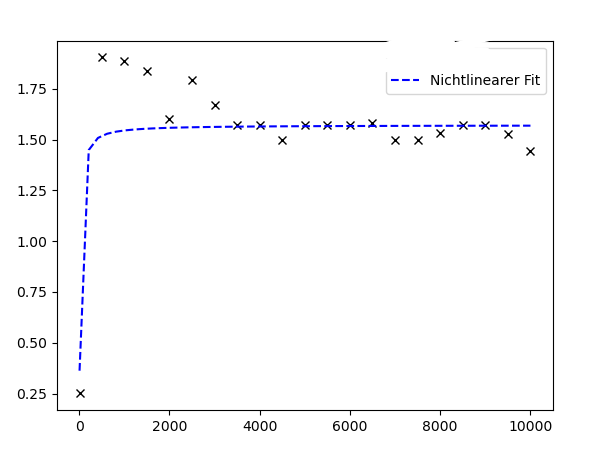
\includegraphics[width=\textwidth]{build/plot1.pdf}
  \caption{Messdaten der Temperaturen}
  \label{fig:plot1}
\end{figure}
\begin{flushleft}
Dabei wurde die Abzisse als Zeit $t$ in Sekunden gewählt. Nun lässt sich eine Ausgleichsfunktion durch
die einzelnen Messwerte legen, dafür wurde hier ein Polynomansatz zweiten Grades gewählt. Also
\end{flushleft}
\begin{equation}
T(t) = \symup{A} t^{2} + \symup{B} t + \symup{C}
\end{equation}
Die Parameter, inklusive Fehler, lassen sich beispielsweise mit einem curvefit in python berechnen.
Für die erste Ausgleichsfunktion $T_{1}$($t$) entstehen folgende Parameter
\begin{align}
\symup{A_{1}} &= (-3.22 \pm 0.042)\cdot 10^{-6} \, \si[per-mode=symbol]{\kelvin\per\second\squared}\\
\symup{B_{1}} &= (20 \pm 0.091) 10^{-3} \,\si[per-mode=symbol]{\kelvin\per\second}\\
\symup{C_{1}} &= (294.97 \pm 0.042) \,\si{\kelvin}
\end{align}
Analog erhält man für die Ausgleichsfunktion $T_{2}$($t$) die Parameter
\begin{align}
\symup{A_{2}} &= (9.55 \pm 2.67)\cdot 10^{-7} \, \si[per-mode=symbol]{\kelvin\per\second\squared}\\
\symup{B_{2}} &= (-11.20 \pm 0.58) 10^{-3} \,\si[per-mode=symbol]{\kelvin\per\second}\\
C_{2} &= (295.87 \pm 0.26) \,\si{\kelvin}
\end{align}
Wenn man diese Funktionen nun in das Diagramm \ref{fig:plot1} einfügt, erkennt man,
dass die Parameter plausibel sind.
\begin{figure}[h]
  \centering
  \includegraphics[width=\textwidth]{build/plot2.pdf}
  \caption{Messdaten der Temperaturen und Ausgleichsfunktionen}
  \label{fig:plot2}
\end{figure}
\begin{flushleft}
Nun kann man sich jeweils vier verschiedene Messpunkte anschauen und die dazugehörigen Differenzenquotienten bestimmen. Dafür wurden hier
Messstellen im Abstand von 400 Sekunden gewählt.
Der Differenzenquotienten des Polynom zweiten Grades lautet wie folgt.
\end{flushleft}
\begin{equation}
\frac{\symup{d}T}{\symup{d}t} = 2 \symup{A} t + \symup{B}
\end{equation}
In den Gleichungen \eqref{eq25} bis \eqref{eq28} sind die ausgerechneten Differenzenquotienten des Temperaturverlaufs $T_{1}$
\begin{align}
\left( \frac{\symup{d}T_{1}}{\symup{d}t}\right)_{400} &= (17.7\pm0.1)\cdot 10^{-3} \, \text{[K/s]} \label{eq25}\\
\left(\frac{\symup{d}T_{1}}{\symup{d}t}\right)_{800} &= (15.1\pm0.1)\cdot 10^{-3} \,\text{[K/s]}\\
\left(\frac{\symup{d}T_{1}}{\symup{d}t}\right)_{1200} &= (12.54\pm0.14)\cdot 10^{-3} \, \text{[K/s]}\\
\left(\frac{\symup{d}T_{1}}{\symup{d}t}\right)_{1600} &= (9.97\pm0.16)\cdot 10^{-3} \, \text{[K/s]} \label{eq28}
\end{align}
Für den zweiten Temperaturverlauf $T_{2}$ erhält man
\begin{align}
\left( \frac{\symup{d}T_{2}}{\symup{d}t}\right)_{400} &= (10.4\pm0.6)\cdot 10^{-3} \, \text{[K/s]} \label{eq29}\\
\left(\frac{\symup{d}T_{2}}{\symup{d}t}\right)_{800} &= (9.7\pm0.7)\cdot 10^{-3} \,\text{[K/s]}\\
\left(\frac{\symup{d}T_{2}}{\symup{d}t}\right)_{1200} &= (8.9\pm0.9)\cdot 10^{-3} \, \text{[K/s]}\\
\left(\frac{\symup{d}T_{2}}{\symup{d}t}\right)_{1600} &= (8.2\pm1.0)\cdot 10^{-3} \, \text{[K/s]} \label{eq32}
\end{align}
Dabei lassen sich die Fehler über die Gaußsche Fehlerfortpflanzung berechnen.
\begin{equation}
  \increment \left( \frac{\symup{d}T}{\symup{d}t}\right) = \sqrt{\left( \frac{\partial}{\partial A} \left( \frac{\symup{d}T}{\symup{d}t} \right)\right)^{2} \cdot (\increment A)^{2} + \left( \frac{\partial}{\partial B} \left( \frac{\symup{d}T}{\symup{d}t} \right)\right)^{2} \cdot (\increment B)^{2} }
  \label{eqn:gaussianmistake}
\end{equation}
\subsection{Berechnung der Güteziffer}
